\subsection{Experiment Results}
\label{sec:res}

\subsubsection{Distribution of article composition: where do humans and agents differ?}
Before examining the article content, a natural first check is whether \methodshort{} writes at human scale. Across the 18 paired articles (Figure~\ref{fig:dist-periods}), the total writing volume comes out roughly comparable (1305 for \methodshort{} and 1557 for humans), while the agent uses $1.45{\times}$ as many sentences but each is shorter ($0.77{\times}$); the articles made by \methodshort{} are broken into shorter, more granular statements.

\begin{figure}[!h]
    \centering
    \begin{subfigure}[t]{0.4\linewidth}
        \centering
        
\includegraphics[width=\linewidth]{exp-meta/dist/periods/fig.pdf}
        \caption{Num. of sentences per article and Avg. words per sentence.}
        \label{fig:dist-periods}
    \end{subfigure}
    % \hfill
    \begin{subfigure}[t]{0.4\linewidth}
        \centering
        
\includegraphics[width=\linewidth]{exp-meta/dist/coverage/fig.pdf}
        \caption{Claim coverage between human-written and agent-generated articles.}
        \label{fig:dist-coverage}
    \end{subfigure}
    \caption{\textbf{Textual distribution (left) and Content coverage (right)} across 18 samples, reported by “mean $\pm$SEM” with p value.}
    \label{fig:dist}
\end{figure}

Matching textual statistics is one thing; the angle behind the text is what matters.
As shown in Figure~\ref{fig:dist-coverage}, claim-level coverage points clearly one way: about half of the human article angle (50.4\%) lands in the agent's article, while only a third (35.1\%) of the agent’s angle maps back. 
We find that the pattern is source-shaped, and each gap has a clear cause: it is widest on `Economist' short briefings ($\Delta=73.0\%-\ 39.5\%=33.5\%$), whose narrow single-topic scope (typically standard statistic or chart) makes them easy for the agent to predict and cover; 
it stays uniformly lower on `Pudding' and `TidyTuesday', whose source articles either carry a single editorial thesis the agent does not fully reproduce (creative long-form storytelling) or span diverse topics as well as external sources (`TidyTuesday').
\methodshort{} reliably absorbs and rewrites the easy, predictable angles, but \textit{reproducing a human author's narrative arc remains the harder problem.}

\begin{figure}[!h]
    \centering
    \begin{subfigure}[t]{0.4\linewidth}
        \centering
        
\includegraphics[width=\linewidth]{exp-meta/multimodal/by_group/fig.pdf}
        \caption{Articles made by \methodshort{}.}
        \label{fig:multimodal-agent-bygroup}
    \end{subfigure}
    % \hfill
    \begin{subfigure}[t]{0.4\linewidth}
        \centering
        
\includegraphics[width=\linewidth]{exp-meta/multimodal/human_by_group/fig.pdf}
        \caption{Articles made by human.}
        \label{fig:multimodal-human-bygroup}
    \end{subfigure}
    \caption{\textbf{Multimodal media asset distributions} (\eg~video, image, audio, interactive, etc) between \methodshort{} (left) and human (right).}
    \label{fig:media}
\end{figure}

% \textbf{Multimedia distribution.}
Beyond text, every article may carry various multimedia assets, leading the article style to diverge sharply. 
We classify multimedia assets by six categories: heading (big short title), interactive, audio, video, image, and chart. 
As illustrated in Figure~\ref{fig:multimodal-agent-bygroup}, \methodshort{}'s media distribution is uniform across all three sources: it averages 13--14 assets per article and covers every modality in similar proportions. 
By contrast, Figure~\ref{fig:multimodal-human-bygroup} shows that human authors tune the kit to the publication: `Pudding' carries about 41 assets per article, rich in video, audio, and interactives, while `The Economist' and `TidyTuesday' stay near 3--4, almost all charts and images. 
\textit{\methodshort{} robustly produces every modality across topics, whereas human designers vary their distribution substantially with editorial style.}


\subsubsection{Human studies as primary testbed}
\paragraph{\methodshort{} articles are appreciated by humans across various rubrics.}
Figure~\ref{fig:judgehuman-dims} reports per-dimension means across the 53 participants, with the agent ahead on all five axes (with an overall mean of $4.21$ for \methodshort{} and $3.38$ for humans). 
The largest gap is on “Transparency” ($+1.49$), a margin we attribute to the Inspector per-sentence provenance and we provide an ablation in §\ref{sec:Inspector}; the smallest is on “Visual” ($+0.51$), which we further ablate next.

\paragraph{Analytical genres amplify the agent's advantage, while editorial scrollytelling narrows it.}
Figure~\ref{fig:judgehuman-bycat} shows the breakdown by source: \textit{Economist} ($\Delta{=}{+}1.02$, $p{<}.001$) and \textit{TidyTuesday} ($\Delta{=}{+}1.20$, $p{<}.001$) both clearly favour the agent, while \textit{Pudding} is a statistical tie. Pudding's long-form scrollytelling pieces are produced by art designer teams who spend weeks per article on bespoke design and a single committed thesis, an authorial investment the agent does not yet match. 
\textit{The agent performs best in genres where analytical framing matters more than authorial voice; in the most designer-curated genre, it merely matches human performance.}

\begin{figure*}[!h]
    \centering
    \begin{subfigure}[t]{0.32\textwidth}
        \centering
        
\includegraphics[width=\linewidth]{exp-meta/judge_human/dim_means/fig.pdf}
        \caption{By rubric dimension.}
        \label{fig:judgehuman-dims}
    \end{subfigure}
    \hfill
    \begin{subfigure}[t]{0.32\textwidth}
        \centering
        
\includegraphics[width=\linewidth]{exp-meta/judge_human/by_category/fig.pdf}
        \caption{By source category.}
        \label{fig:judgehuman-bycat}
    \end{subfigure}
    \hfill
    \begin{subfigure}[t]{0.32\textwidth}
        \centering
        
\includegraphics[width=\linewidth]{exp-meta/judge_human/preference/fig.pdf}
        \caption{Overall pairwise preference.}
        \label{fig:judgehuman-pref}
    \end{subfigure}
    \caption{\textbf{Human evaluation ($n{=}53$ reviewers).} Scores are grouped by rubric dimension (a) and source category (b). Finally, reviewers were asked to choose the better article through pairwise comparisons (c).}
\label{fig:judgehuman}
\end{figure*}

\paragraph{The holistic preference is consistent with the rubric.}
Beyond the per-dimension scores, each reviewer also gave a single overall preference after seeing both versions. Figure~\ref{fig:judgehuman-pref} shows the result: of the $53$ reviewers, $39$ preferred \methodshort{}, $13$ preferred the human version, and $1 (2\%)$ calling it a tie. 
The holistic preference moves in the same direction as the per-dimension rubric, which suggests that the dimensions the rubric isolates (transparency, claim-data alignment, and so on) are also the ones reviewers weigh when forming an overall judgment. 

\subsubsection{Computer-use agent as a cost-efficient alternative}
Figure~\ref{fig:judgevlmcodex-avg} reports the Agent judge's average score with ablation of the Inspector across the three sources. %1
% \kevin{
Notably, we treat the agent judge as a cost-efficient proxy for ranking articles rather than a major quality signal; quality claims rest on the human study alone.
% }
\paragraph{Transparency's Inspector lift is roughly $2.5{\times}$ the next-largest dimension and dwarfs the rest.}
With the Inspector off, the agent's overall mean is $4.60$ (human reference: $3.87$), and on \textit{Pudding} the two are identical ($4.90$ each), consistent with the human study. Opening the Inspector raises the overall mean to $5.10$, a further $\sim{}0.50$.
Figure~\ref{fig:judgevlmcodex-dims} breaks the same three conditions down by rubric dimension: the effect concentrates almost entirely on \emph{3-Transparency} ($4.28{\to}5.94$, $\Delta{=}{+}1.67$), with \emph{4-Claim} a distant second ($\Delta{=}{+}0.67$) and the remaining three dimensions barely shifting ($\Delta{\le}0.11$).
The Inspector thus buys a single dominant transparency channel plus a modest claim--data assist, with little spillover onto visual, narrative, or insight.

% 2
\paragraph{The agent judge preserves the human ranking at a fraction of the cost.}
A practical question is whether the cheaper agent judge can stand in for the 53-reviewer study on the same articles. The two judges rank articles together ($\rho{=}0.44$, $p{<}.01$;
Figure~\ref{fig:judgevlmcodex-agree}), and almost every point ($29{/}34$) sits above the $y{=}x$ line, so the agent keeps the human ordering while scoring both \methodshort{} and human articles higher in absolute terms.
\textbf{The agent judge is a usable stand-in for the ranking the human study produces, at a fraction of the cost.}


\begin{figure*}[t]
    \centering
    \begin{subfigure}[t]{0.32\textwidth}
        \centering
        
\includegraphics[width=\linewidth]{exp-meta/judge_vlm_codex/avg/fig.pdf}
        \caption{By source category.}
        \label{fig:judgevlmcodex-avg}
    \end{subfigure}
    \hfill
    \begin{subfigure}[t]{0.32\textwidth}
        \centering
        
\includegraphics[width=\linewidth]{exp-meta/judge_vlm_codex/dims/fig.pdf}
        \caption{By rubric dimension.}
        \label{fig:judgevlmcodex-dims}
    \end{subfigure}
    \hfill
    \begin{subfigure}[t]{0.32\textwidth}
        \centering
        
\includegraphics[width=\linewidth]{exp-meta/judge_vlm_codex/judge_agreement/fig.pdf}
        \caption{Agent judge aligns with human judge.}
        \label{fig:judgevlmcodex-agree}
    \end{subfigure}
    \caption{\textbf{Agent-as-judge evaluation.} Scores are compared across \methodshort{} articles with the Inspector, \methodshort{} articles without the Inspector, and human-written articles. Results are grouped by source category (a) and rubric dimension (b), with score distributions from agent-judge and human-judge compared in (c).}
    \label{fig:judgevlmcodex}
\end{figure*}

\subsubsection{Verifiability analysis: auditability rather than factuality}
Figure~\ref{fig:repro} (a,b) reports machine-checkable provenance coverage across publication sources.
For \methodshort{} articles, 93\% of visible claims resolve to a traceable binding between the rendered text and its upstream evidence.
Human reference articles ship no accompanying code, so by construction most claims cannot be checked this way; the Codex verifier has to guess at a plausible reproduction on its own from the raw data and the published text alone.
Thus, text-only audit recovers such a binding for 25\% of claims. This makes sense as human-written statements are written for general readers and rarely attach a line of code or a traceable source to each claim, whereas our Inspector question bank probes for exactly that.
It is worth noting that \textbf{they measure whether a claim carries a verifiable provenance trail, not whether it is factually correct.}
The gap therefore reflects the availability of machine-checkable provenance, not the quality of human journalism.


% Figure~\ref{fig:repro-bycat} aggregates pass rates across different publication sources.
% The \methodshort{} article pass at 93\% against 25\% for the human reference;
% we emphasise that this metric distinguishes \textit{auditability} from \textit{factual correctness}: 
% the disparity does not imply that human-written statements are less factually correct. Rather, human articles are written for general readers and rarely accompany every claim with a line of code or a traceable source, whereas our Inspector question bank explicitly probes them.
% The reproducibility gap therefore largely measures the \textit{availability of traceable provenance rather than the quality of human journalism}. This highlights \methodshort{}'s capacity to produce highly auditable articles in 
% which claims are aligned with the underlying data by construction.

\begin{figure}[!h]
    \centering
    \begin{subfigure}[t]{0.32\textwidth}
        \centering
        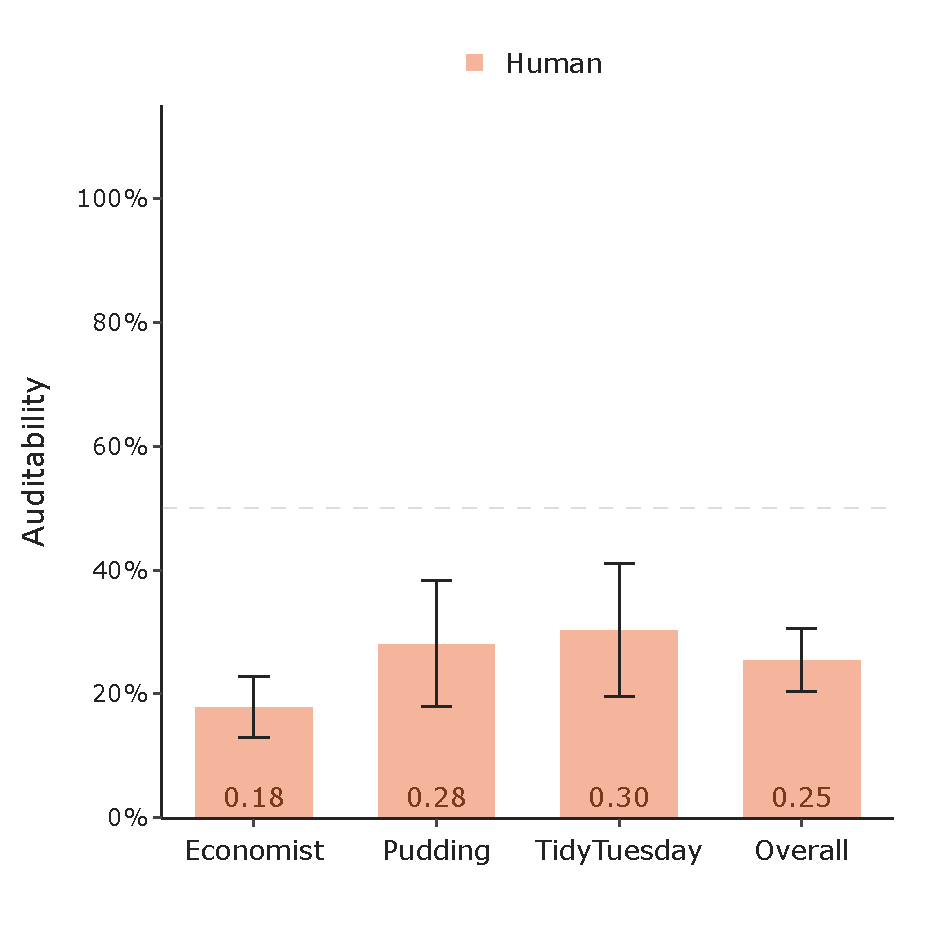
\includegraphics[width=\linewidth]{exp-meta/repro/by_category_sep/fig_human.pdf}
        \caption{Human, per source.}
        \label{fig:repro-bycat-human}
    \end{subfigure}
    \begin{subfigure}[t]{0.32\textwidth}
        \centering
        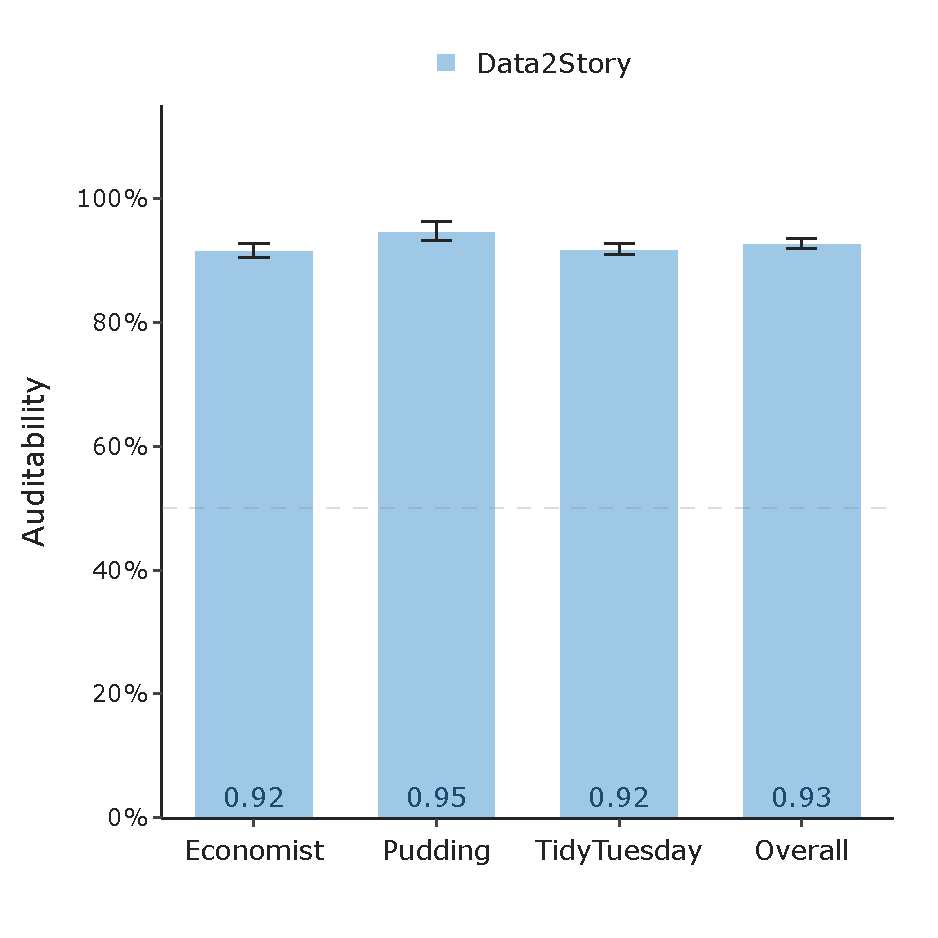
\includegraphics[width=\linewidth]{exp-meta/repro/by_category_sep/fig_ours.pdf}
        \caption{\methodshort, per source.}
        \label{fig:repro-bycat-ours}
    \end{subfigure}
    \begin{subfigure}[t]{0.32\textwidth}
        \centering
        
\includegraphics[width=\linewidth]{exp-meta/repro/scatter_ecdf/fig.pdf}
        \caption{Empirical CDF over all 18 articles.}
        \label{fig:repro-ecdf}
    \end{subfigure}
    \caption{\textbf{Auditability between \methodshort-generated and human-written articles.} Per-source means with SEM error bars for human (a) and \methodshort{} (b); empirical CDF over all 18 articles (c).}
    \label{fig:repro}
\end{figure}

All three sources show a wide and significant gap. The gap is narrowest for {Economist}, whose briefing-style articles foreground more explicit and standard numerical analysis. This makes the likely human findings easier to anticipate, because many insights can be inferred from visible statistics, comparisons, and trends. In contrast, the gap is widest for {Pudding}, whose scrollytelling pieces often center on creative editorial ideas and qualitative framing rather than enumerated sub-population statistics. These ideas are less formulaic and therefore harder to guess from the pre-registered questions alone. 

Figure~\ref{fig:repro-ecdf} shows the empirical distribution of article auditability. \methodshort{} articles concentrate in a tight band near the top of the auditability axis, while the human distribution is spread more broadly. This suggests that the auditability that \methodshort{} offers is largely the pipeline itself rather than of any particular reference article; claims are bound to upstream evidence by construction, whereas in human’s articles the same kind of binding only appears when the author chose to expose it.

\begin{figure}[!h]
    \centering
    \begin{subfigure}[t]{0.28\linewidth}
        \centering
        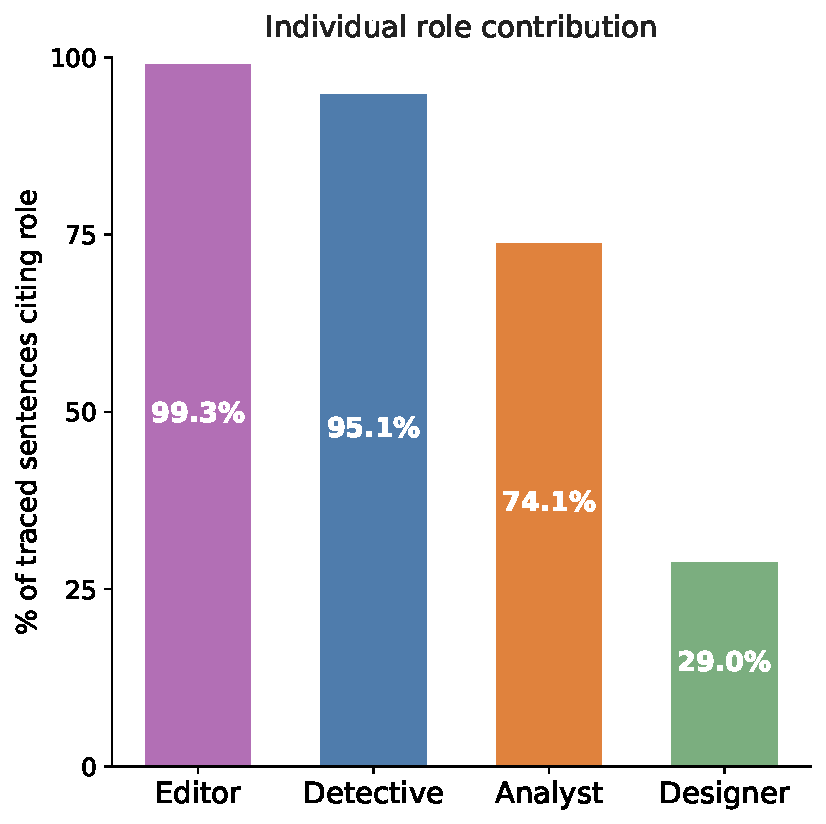
\includegraphics[width=\linewidth]{exp-meta/ablation_role/overall/fig.pdf}
        \caption{Individual role contribution.}
    \label{fig:Inspector-diff}
    \end{subfigure}
    \begin{subfigure}[t]{0.32\linewidth}
        \centering
        
\includegraphics[width=\linewidth]{exp-meta/judge_human/inspector/selfreport/fig.pdf}
    \caption{Human participants' votes on whether the Inspector was useful.}
    \label{fig:Inspector-selfreport}
    \end{subfigure}
    \begin{subfigure}[t]{0.32\linewidth}
        \centering
        
\includegraphics[width=\linewidth]{exp-meta/judge_vlm_codex/panel_effect/fig.pdf}
        \caption{Within-article Inspector effect on different rubrics.}
        \label{fig:Inspector-paneleffect}
    \end{subfigure}
    \caption{\textbf{Analysis of Inspector effect.} Human participants' usefulness ratings of the Inspector (a), and Agent judges inspector-related gains across rubric dimensions (b).}
    \label{fig:Inspector}
\end{figure}

% \subsubsection{Ablation of Inspector}
\subsubsection{Analysis of different roles}
\label{sec:Inspector}
The inspector subagent exposes the per-sentence provenance produced by four different roles: {Detective} (sourcing), {Analyst} (computation), {Designer} (chart authoring), and {Editor} (storytelling). Figure~\ref{fig:Inspector-diff} reports per-role coverage across all articles: \textit{Editor} $99.3\%$, \textit{Detective} $95.1\%$, \textit{Analyst} $74.1\%$ and \textit{Designer} $29.0\%$. These shares reflect each role's working character more than the data itself: Editor and Detective participate in nearly every traced sentence --- every claim is storyboarded, and Detective's search-heavy sourcing names at least one external reference; Analyst adds computation to roughly three quarters of sentences (the quantitative subset); Designer is selective, anchoring visual assets in about a third.

\textbf{Effect of Inspector.}
Figure~\ref{fig:Inspector-selfreport} reports how the $n{=}53$ reviewers experienced the Inspector, which attaches per-claim provenance information including analyst notes, code-line references, and source datasets---to the rendered article. 
Overall, $66\%$ of participants found the Inspector helpful for forming their evaluations, only $3 (6\%)$ rated it not helpful, whereas $25\%$ found it unhelpful or distracting. The main concern was that the provenance traces were sometimes dense and complex, linking each claim to multiple scripts, quoted sources, and data references.

Figure~\ref{fig:Inspector-paneleffect} isolates the Inspector behavioral effect: same article, same computer-use agent judge, only difference is whether the Inspector is open. The within-pair lift concentrates on \emph{3-Transparency} ($\Delta{=}{+}1.67$, paired, $p{<}.001$). This further highlights that \textit{opening the Inspector lifts mainly the transparency rubric}.

\subsection{Qualitative assessment: where human did better?}
We examine individual examples from each publication source, comparing the articles produced by \method~with those written by human journalists. 
This qualitative view surfaces values that our numerical experiments miss. 
Across the paired set, the human edge shows up in three recurring forms: the editorial angle, the creative design, and the informative presentation.

\textbf{(i) Editorial Angle.}
The human advantage we could not close is the angle that comes from outside the data. The Repair Cafés reporter (Table~\ref{tab:caseT4-opening}) frames repair as a matter of accountability, attributing failure to manufacturers that build ``phones, cars and tractors'' so that mechanics cannot access ``diagnostic tools or broken parts'' without them. Such a claim is reported rather than computed: it rests on expert testimony and on outside knowledge the dataset never holds. Working only from the table, \methodshort{} can rank what breaks (knives are saved far more often than printers), but it leaves the cause to the reader. This is the qualitative face of our coverage finding (\S\ref{sec:res}). Across the paired set the agent recovers only about half of the human's editorial angle, because the other half lives in reporting it cannot reach.

\textbf{(ii) Creative Design.}
On the \textit{Pudding} pieces, human teams invest weeks of bespoke interaction the agent does not attempt. The Stand-Up Comedy article (Table~\ref{tab:caseP1-opening}) turns the transcript into the interface: ``every line'' of Ali Wong's special is on the page, and each laugh is marked beside its line as a circle scaled to its length. For the same material, \methodshort{} links out to a static YouTube thumbnail and summarises the set in standard charts. A similar gap appears in the Internet Boy Band Database (Table~\ref{tab:caseP4-opening}), which plays as an audio-visual jukebox of all $55$ acts, its hand-animated members morphing from band to band as each act's song plays; the agent re-tells the same history in static charts behind click-to-play embeds. The numbers survive, but not the crafted experience built around them.

\textbf{(iii) Informative Presentation.}
Even in a single static figure, human designers carry more meaning per frame. The space-race chart (Table~\ref{tab:caseE1-opening}) sets state against commercial launch providers on one timeline and folds in a second variable for free: each band is shaded lighter where launches failed, with an annotation explaining why the Soviet count runs so high. Its satellites ``lasted only a year and a half on average, compared with nine years for their American counterparts.'' \methodshort{} distributes the same material across many single-variable charts, so no one figure carries the story. The football-managers chart (Table~\ref{tab:caseE3-opening}) overlays managers and star players on one axis, placing Messi and Ronaldo at the high end where the chart's own annotation reads: ``Star players' impact can reach ten points per season. Managers rarely add more than two.'' Our agent plots only the managers, and the comparison the headline promises never appears.

These cases show that the human contribution should not be understated. \methodshort{} leads on coverage, analysis, and auditable transparency, yet the reported angle, together with the hand-built craft behind a design or a chart, remains a human strength.